\section{Knoten}
\begin{frame}{}
    \begin{center}
        Freifunk Franken Knoten
     \end{center}
\end{frame}

\begin{frame}{Freifunk Franken Knoten}
    \begin{center}
        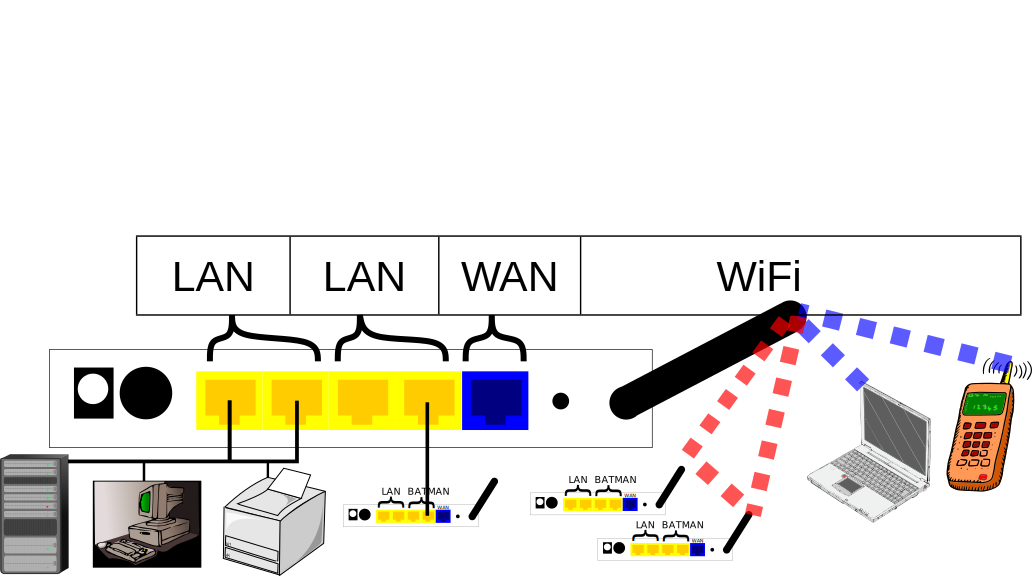
\includegraphics[width=0.75\textwidth]{img/svg/anschluesse.pdf}
    \end{center}
    \begin{tabular}{ll}
        LAN, Access-Point: & Client-Ports\footnote{,,Wie ein großer Switch''} \\
        Batman, Ad-Hoc: & Mesh-Netz \\
        WAN: & VPN Zugang \\
    \end{tabular}
\end{frame}

\begin{frame}{Interner Aufbau}
    \begin{itemize}
        \item OpenWrt
        \item Batman-Adv
        \item Fastd Client
        \item Monitoring Daten (Nodewatcher / Alfred)
        \item .. kleinere Tools / Configs / Skripte
    \end{itemize}

    \renewcommand{\arraystretch}{1.5}
    \begin{tabular}{|c|c|c|c|c|c|c|} \hline
         \multicolumn{7}{|c|}{Bridge} \\ \hline
         \multirow{2}{*}{Managed} &
         \multicolumn{4}{c|}{B.A.T.M.A.N} &
         \multicolumn{2}{c|}{\multirow{2}{*}{Client-VLan}} \\ \cline{2-5}
         & Ad-Hoc & VPN & \multicolumn{2}{c|}{Node-VLan} & \multicolumn{2}{c|}{} \\ \hline
         \multicolumn{2}{|c|}{WiFi} & WAN & LAN1 & LAN2 &
         LAN3 & LAN4 \\ \hline
    \end{tabular}
\end{frame}

\begin{frame}{Freifunk Knoten}
    \only<1>{
        \begin{itemize}
            \item Vergibt ein spezielles IPv6 Prefix: fdff:0::
            \begin{itemize}
                \item fdff:0::1
                \item fdff:0::\$\{MAC\}
                \item fdff:0::\$\{Link-Local suffix\}
            \end{itemize}
            \item Webinterface
            \item Konfiguration am Gerät
            \begin{itemize}
                \item Passwort
                \item Knoten-Name
                \item Beschreibung
                \item Ansprechpartner
                \item Standort
            \end{itemize}
        \end{itemize}
    }
    \only<2-4>{\hspace{-0.04\textwidth}
        \noindent\fbox{\noindent
            \only<2>{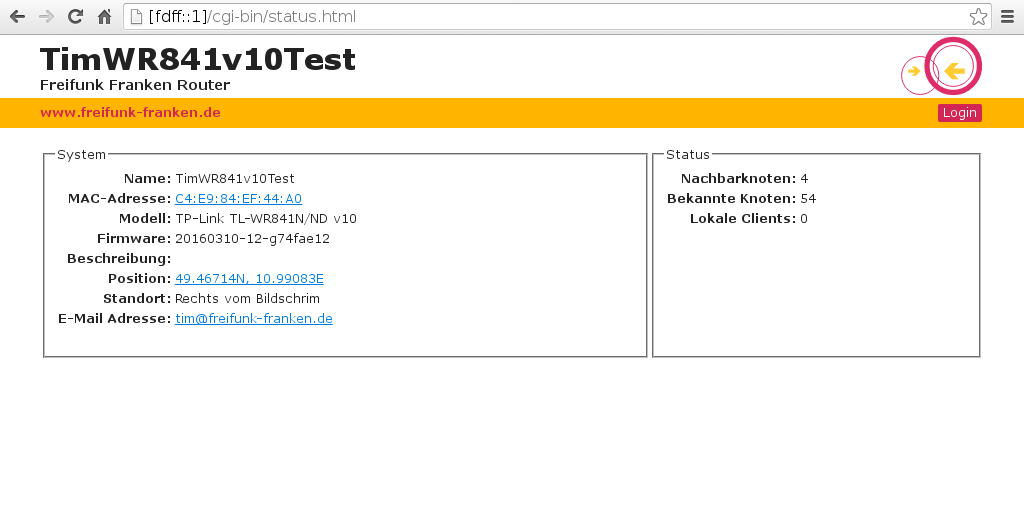
\includegraphics[width=1.03\dimexpr\textwidth-2\fboxsep-2\fboxrule\relax]{img/web-if-1.png}}%
            \only<3>{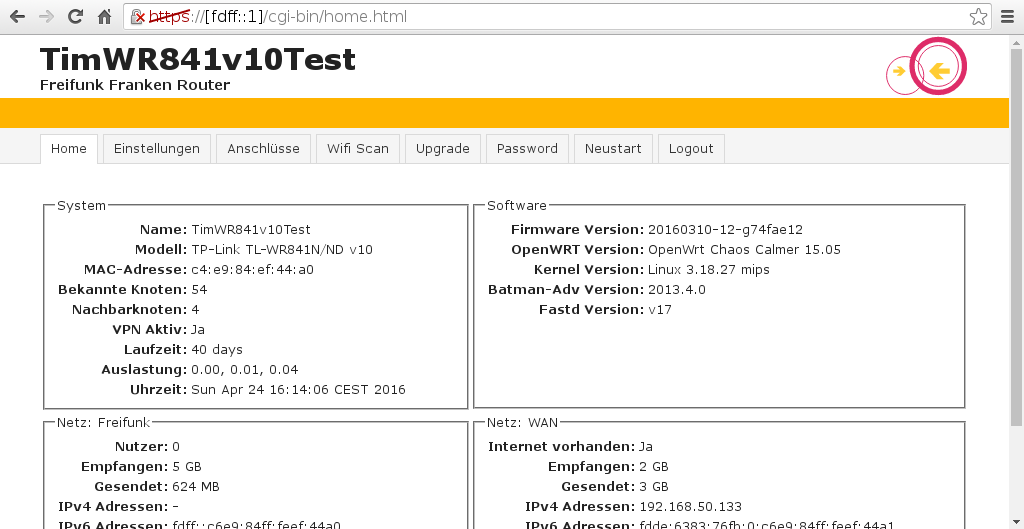
\includegraphics[width=1.03\dimexpr\textwidth-2\fboxsep-2\fboxrule\relax]{img/web-if-2.png}}%
            \only<4>{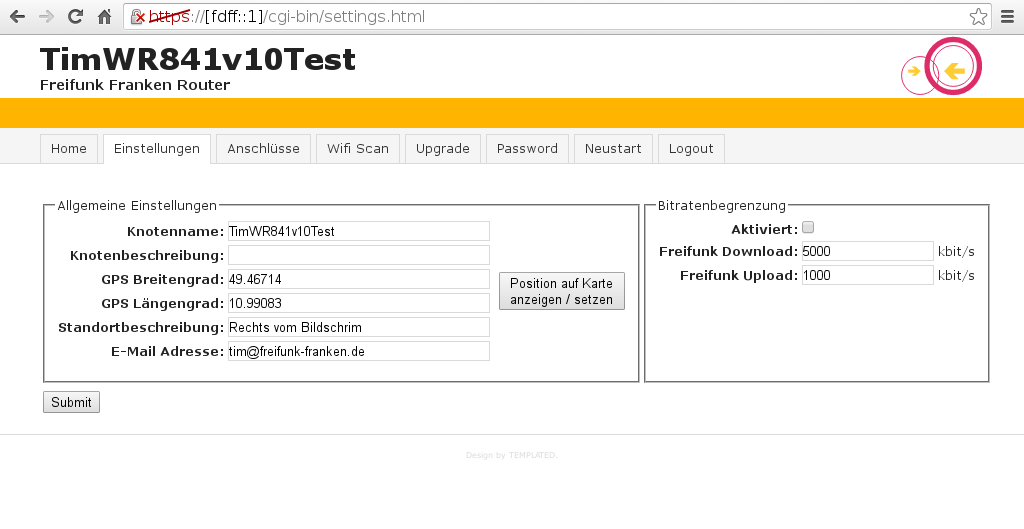
\includegraphics[width=1.03\dimexpr\textwidth-2\fboxsep-2\fboxrule\relax]{img/web-if-3.png}}%
        }
    }
\end{frame}
